\section{Dos memorias independientes}

La CPU utiliza dos memorias lógicamente independientes, cada una con su propio
contenido y recorrido de acceso:

\begin{itemize}
  \item \textbf{\tech{IMEM}:} conserva la imagen confirmada de instrucciones
    que IF puede buscar durante la ejecución.
  \item \textbf{\tech{DMEM}:} conserva los datos de la sesión sobre los que
    operan las instrucciones de load y store.
\end{itemize}

Ambas comienzan en la dirección \code{0x00000000}, pero no comparten el mismo
espacio de direcciones. Por eso, una dirección numérica igual puede identificar
una posición de IMEM y otra distinta de DMEM.

La separación permite que IF lea una instrucción mientras MEM accede a los datos
en el mismo ciclo. No se produce un hazard estructural entre el fetch y el
acceso a datos, y cada memoria recibe como máximo una solicitud de la CPU por
ciclo. El contrato completo se encuentra en
\doc{architecture/memory/memory_architecture.md}{Arquitectura de memoria}.

\begin{figure}[H]
  \centering
  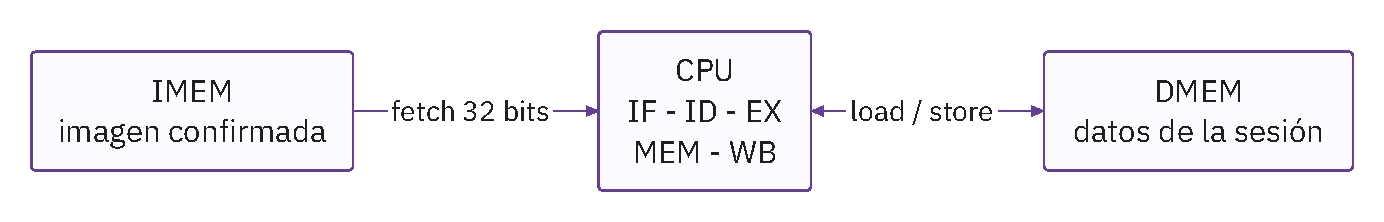
\includegraphics[width=0.95\textwidth]{memorias.pdf}
  \caption{Espacios independientes de instrucciones y datos.}
  \label{fig:memorias}
\end{figure}

\section{Instruction Memory}

IMEM almacena la imagen de instrucciones que utiliza el procesador. Es una
memoria direccionada por bytes: el PC representa la dirección del primer byte
del fetch y cada instrucción ocupa cuatro direcciones consecutivas, \code{PC},
\code{PC + 1}, \code{PC + 2} y \code{PC + 3}. Por ejemplo, si
\code{PC = 0x08}, la instrucción se forma con los bytes de \code{0x08} a
\code{0x0B}.

Durante la ejecución, la lectura de IMEM es combinacional mientras que durante la carga, la
escritura es síncrona. Ninguna de las dos operaciones agrega una latencia
variable ni un stall específico de memoria.

\subsection{Imagen ejecutable}

En este capítulo, llamaremos a una \emph{imagen} como el conjunto de bytes de programa que la
PC envía mediante \code{LOAD} y que el sistema recibe y escribe en IMEM. La imagen incluye solo el tramo cargado del programa:
su tamaño se conserva en \code{loaded_image_size_bytes} y ese límite determina
qué bytes pueden buscarse como instrucciones.

La imagen ejecutable es una única región inicial y continua. Para que pueda
publicarse, debe cumplir todas estas condiciones:

\begin{itemize}
  \item comienza en \code{0x00000000};
  \item no está vacía;
  \item no tiene huecos;
  \item su tamaño es múltiplo de cuatro;
  \item no supera \code{IMEM_CAPACITY_BYTES}.
\end{itemize}

Una sesión preparada comienza a ejecutar desde \code{PC = 0}, el inicio de la
imagen. El tamaño confirmado se conserva en \code{loaded_image_size_bytes}; de
ese valor se derivan \code{image_valid} y la cantidad de instrucciones
disponibles.

La región ejecutable comienza en la dirección cero y termina en el último byte
del tamaño confirmado. Solo los fetches completamente contenidos en ese
intervalo pueden ingresar al pipeline. El contenido físico que quede fuera del
límite no pertenece a la imagen vigente.

\subsection{Validación de fetch}

Para que un fetch sea válido deben cumplirse tres condiciones:

\begin{itemize}
  \item el PC debe estar alineado a cuatro bytes;
  \item los cuatro bytes deben caber dentro de la capacidad física de IMEM;
  \item los cuatro bytes deben pertenecer al tramo confirmado de la imagen.
\end{itemize}

La condición de rango se expresa como:

\begin{codebox}
if_fetch_range_valid =
    image_valid
    && ({1'b0, PC} + 33'd4 <= IMEM_CAPACITY_BYTES)
    && ({1'b0, PC} + 33'd4 <= loaded_image_size_bytes)
\end{codebox}

La comparación utiliza aritmética de 33 bits para conservar el extremo completo
del acceso y evitar que una dirección fuera de rango haga alias con una dirección
baja. Si la validación falla, IF genera un candidato de fault de fetch; ID lo
confirma después de respetar el orden de las instrucciones anteriores.

\subsection{Carga y publicación}

\subsubsection{Recepción y escritura}

El \code{Loader} recibe la imagen byte a byte y reconstruye cada palabra de
cuatro bytes. Durante el proceso de carga conserva los tres primeros bytes que le llegan en un registro de 24 bits y, al
recibir el cuarto, forma la palabra y la escribe en IMEM. La escritura solo se
habilita cuando el \code{Loader} posee la memoria y el índice de palabra es
válido.

\subsubsection{Fin de la carga}

La señal \code{load_ok} certifica que la última palabra se escribió en el
flanco de la última entrega válida. Este evento indica que terminó la
transferencia y la escritura de IMEM; la imagen todavía no es ejecutable.

\subsubsection{Publicación de la imagen}

La imagen se publica cuando termina la preparación de la sesión. En el flanco
que consume \code{prepare_done}, el sistema captura el tamaño validado en
\code{loaded_image_size_bytes}. A partir de ese momento, ese tamaño delimita
los fetches que pueden considerarse parte de la imagen ejecutable.

Si la carga o la preparación no terminan correctamente, no se publica una
imagen nueva. Una solicitud \code{LOAD} rechazada conserva la imagen y la
sesión anteriores.

\section{Data Memory}

DMEM almacena los datos que utiliza el programa durante la sesión. La etapa MEM
accede a ella mediante loads y stores de uno, dos o cuatro bytes, según la
instrucción. Está direccionada por bytes, de manera que cada dirección
identifica una posición de un byte.

La lectura es combinacional, por lo que el dato queda disponible sin esperar
un flanco de reloj adicional. En cambio, un store autorizado actualiza los
bytes correspondientes en un flanco de reloj.

Cada byte tiene una marca de validez que indica si fue escrito durante la
sesión actual. Al preparar una nueva sesión se limpian estas marcas y, a medida
que los stores escriben datos, se activan las correspondientes a los bytes
modificados. Así, la lectura devuelve el dato almacenado cuando su marca está
activa y cero cuando está inactiva, aunque físicamente quede un valor de una
sesión anterior.

\subsection{Lanes y little-endian}

Los bytes de DMEM se organizan en filas de cuatro posiciones. Cada posición de
una fila se denomina \emph{lane} y almacena un byte con su correspondiente
marca de validez. Para ubicar una dirección de byte, los dos bits menos
significativos seleccionan el lane y los bits restantes identifican la fila:

\begin{codebox}
lane = direccion[1:0]
fila = direccion >> 2
\end{codebox}

Por ejemplo, las direcciones \code{0x04}, \code{0x05}, \code{0x06} y
\code{0x07} pertenecen a la fila 1 y corresponden, respectivamente, a los
lanes 0, 1, 2 y 3. Esta organización permite leer los cuatro bytes de una fila
como una palabra de 32 bits y seleccionar los bytes que necesita un load. Para
un store, permite identificar los lanes que deben actualizarse.

Los valores de varios bytes se almacenan en orden \emph{little-endian}: el
byte menos significativo ocupa la dirección más baja. Por ejemplo, al
almacenar la palabra \code{0x12345678} desde la dirección $A$, sus bytes
quedan distribuidos de la siguiente manera:

\begin{table}[H]
  \centering
  \small
  \begin{tabular}{cc}
    \toprule
    \textbf{Dirección} & \textbf{Byte} \\
    \midrule
    \code{A + 0} & \code{0x78} \\
    \code{A + 1} & \code{0x56} \\
    \code{A + 2} & \code{0x34} \\
    \code{A + 3} & \code{0x12} \\
    \bottomrule
  \end{tabular}
  \caption{Orden little-endian de un valor de 32 bits.}
  \label{tab:little-endian}
\end{table}

La figura~\ref{fig:memoria-organizacion} muestra, a la derecha, las filas y
lanes de DMEM. La fila resaltada representa el ejemplo anterior con
\code{A = 0x04}, y los círculos indican la validez de cada byte. A la izquierda
se muestra la organización de IMEM para comparar ambas memorias.

\begin{figure}[H]
  \centering
  \begin{tikzpicture}[
      cell/.style={draw=codeviolet, fill=codeback, rounded corners=1pt,
        minimum width=1.22cm, minimum height=0.70cm, inner sep=1pt,
        font=\ttfamily\footnotesize, anchor=center},
      title/.style={font=\small\bfseries, anchor=center},
      note/.style={font=\footnotesize, anchor=center},
      rowlabel/.style={font=\ttfamily\footnotesize, anchor=east},
      valid/.style={circle, draw=codeviolet, fill=codeviolet,
        minimum size=2.4pt, inner sep=0pt},
      invalid/.style={circle, draw=codeviolet, fill=white,
        minimum size=2.4pt, inner sep=0pt},
      arrow/.style={-{Latex[length=2mm]}, thick, draw=codeviolet}
    ]
    % (a) IMEM: palabras de 32 bits, direccionadas por PC >> 2.
    \node[title] at (2.05,1.45) {(a) IMEM};
    \node[note] at (2.05,1.05) {256 palabras de 32 bits};
    \foreach \i/\label in {0/+0, 1/+1, 2/+2, 3/+3} {
      \node[note] at ({0.5+\i*1.3},0.52) {\label};
      \node[cell] (im\i) at ({0.5+\i*1.3},0) {b\i};
    }
    \node[note, anchor=east] at (-0.15,0) {PC};
    \node[note] at (2.05,-0.90) {palabra de 32 bits};
    \node[note] at (2.05,-1.30) {índice de palabra = \code{PC >> 2}};

    % (b) DMEM: cuatro lanes de bytes y una marca de validez por byte.
    \node[title] at (9.95,1.45) {(b) DMEM};
    \node[note] at (9.95,1.05) {4 lanes de bytes $\times$ 512 filas};
    \foreach \lane/\label in {0/0, 1/1, 2/2, 3/3} {
      \node[note] at ({8.15+\lane*1.30},0.52) {lane \label};
    }
    \foreach \row/\addr/\ba/\bb/\bc/\bd/\validflag in {
        0/0x0000/00/00/00/00/0,
        1/0x0004/78/56/34/12/1,
        2/0x0008/00/00/00/00/0,
        3/0x000C/00/00/00/00/0
      } {
        \node[rowlabel] at (7.55,{-\row*1.05}) {\addr};
        \foreach \lane/\cellvalue in {0/\ba, 1/\bb, 2/\bc, 3/\bd} {
          \node[cell] at ({8.15+\lane*1.30},{-\row*1.05}) {\cellvalue};
          \node[invalid] at ({7.75+\lane*1.30},{-\row*1.05+0.23}) {};
        }
      }
    \foreach \lane in {0, 1, 2, 3} {
      \node[valid] at ({7.75+\lane*1.30},{-0.82}) {};
    }
    \draw[codeviolet, thick, rounded corners=2pt] (7.45,-1.50) rectangle (12.75,-0.60);
    \node[note, anchor=west] at (13.15,-1.05) {$A=0x0004$};
  \end{tikzpicture}
  \caption{Organización de las memorias. Cada celda representa un byte; en
  DMEM, el círculo superior izquierdo indica la validez de ese byte: lleno si
  fue escrito y vacío si todavía se lee como cero. La fila resaltada muestra la
  palabra \code{0x12345678} almacenada en \code{0x0004}.}
  \label{fig:memoria-organizacion}
\end{figure}


Los lanes describen la organización lógica de DMEM; la implementación
utiliza arrays inferidos para representar los datos y sus marcas.

\subsection{Loads y stores}

Los loads y stores acceden a DMEM a partir de una dirección efectiva calculada
en EX. En esa etapa también se comprueba la alineación y el rango del acceso,
de modo que MEM recibe las operaciones válidas junto con la información
necesaria para leer o escribir los bytes solicitados.

\subsubsection{Lectura mediante loads}

Para un load, DMEM entrega los cuatro bytes lógicos de la fila que contiene la
dirección efectiva. Por ejemplo, si la dirección es \code{0x05}, la memoria
entrega la fila que abarca las direcciones \code{0x04} a \code{0x07}. Luego,
\code{Load Select/Extend} utiliza los dos bits inferiores de la dirección para
identificar la posición inicial y selecciona uno, dos o cuatro bytes según la
instrucción.

El resultado debe ocupar 32 bits para continuar hacia writeback. En los loads
de uno o dos bytes, el bloque completa los bits superiores con ceros o con
copias del bit de signo, según corresponda. La tabla~\ref{tab:loads} resume
los tamaños y las extensiones de cada instrucción:

\begin{table}[H]
  \centering
  \small
  \begin{tabular}{lll}
    \toprule
    \textbf{Instrucción} & \textbf{Bytes} & \textbf{Resultado} \\
    \midrule
    \code{LB}  & 1 & extensión con signo \\
    \code{LBU} & 1 & extensión con cero \\
    \code{LH}  & 2 & ensamblado y extensión con signo \\
    \code{LHU} & 2 & ensamblado y extensión con cero \\
    \code{LW}  & 4 & palabra completa \\
    \bottomrule
  \end{tabular}
  \caption{Selección y extensión de loads.}
  \label{tab:loads}
\end{table}

La figura~\ref{fig:mem-load} muestra este recorrido, desde la lectura de DMEM
hasta la selección y extensión del valor que continúa hacia writeback.

\begin{figure}[H]
  \centering
  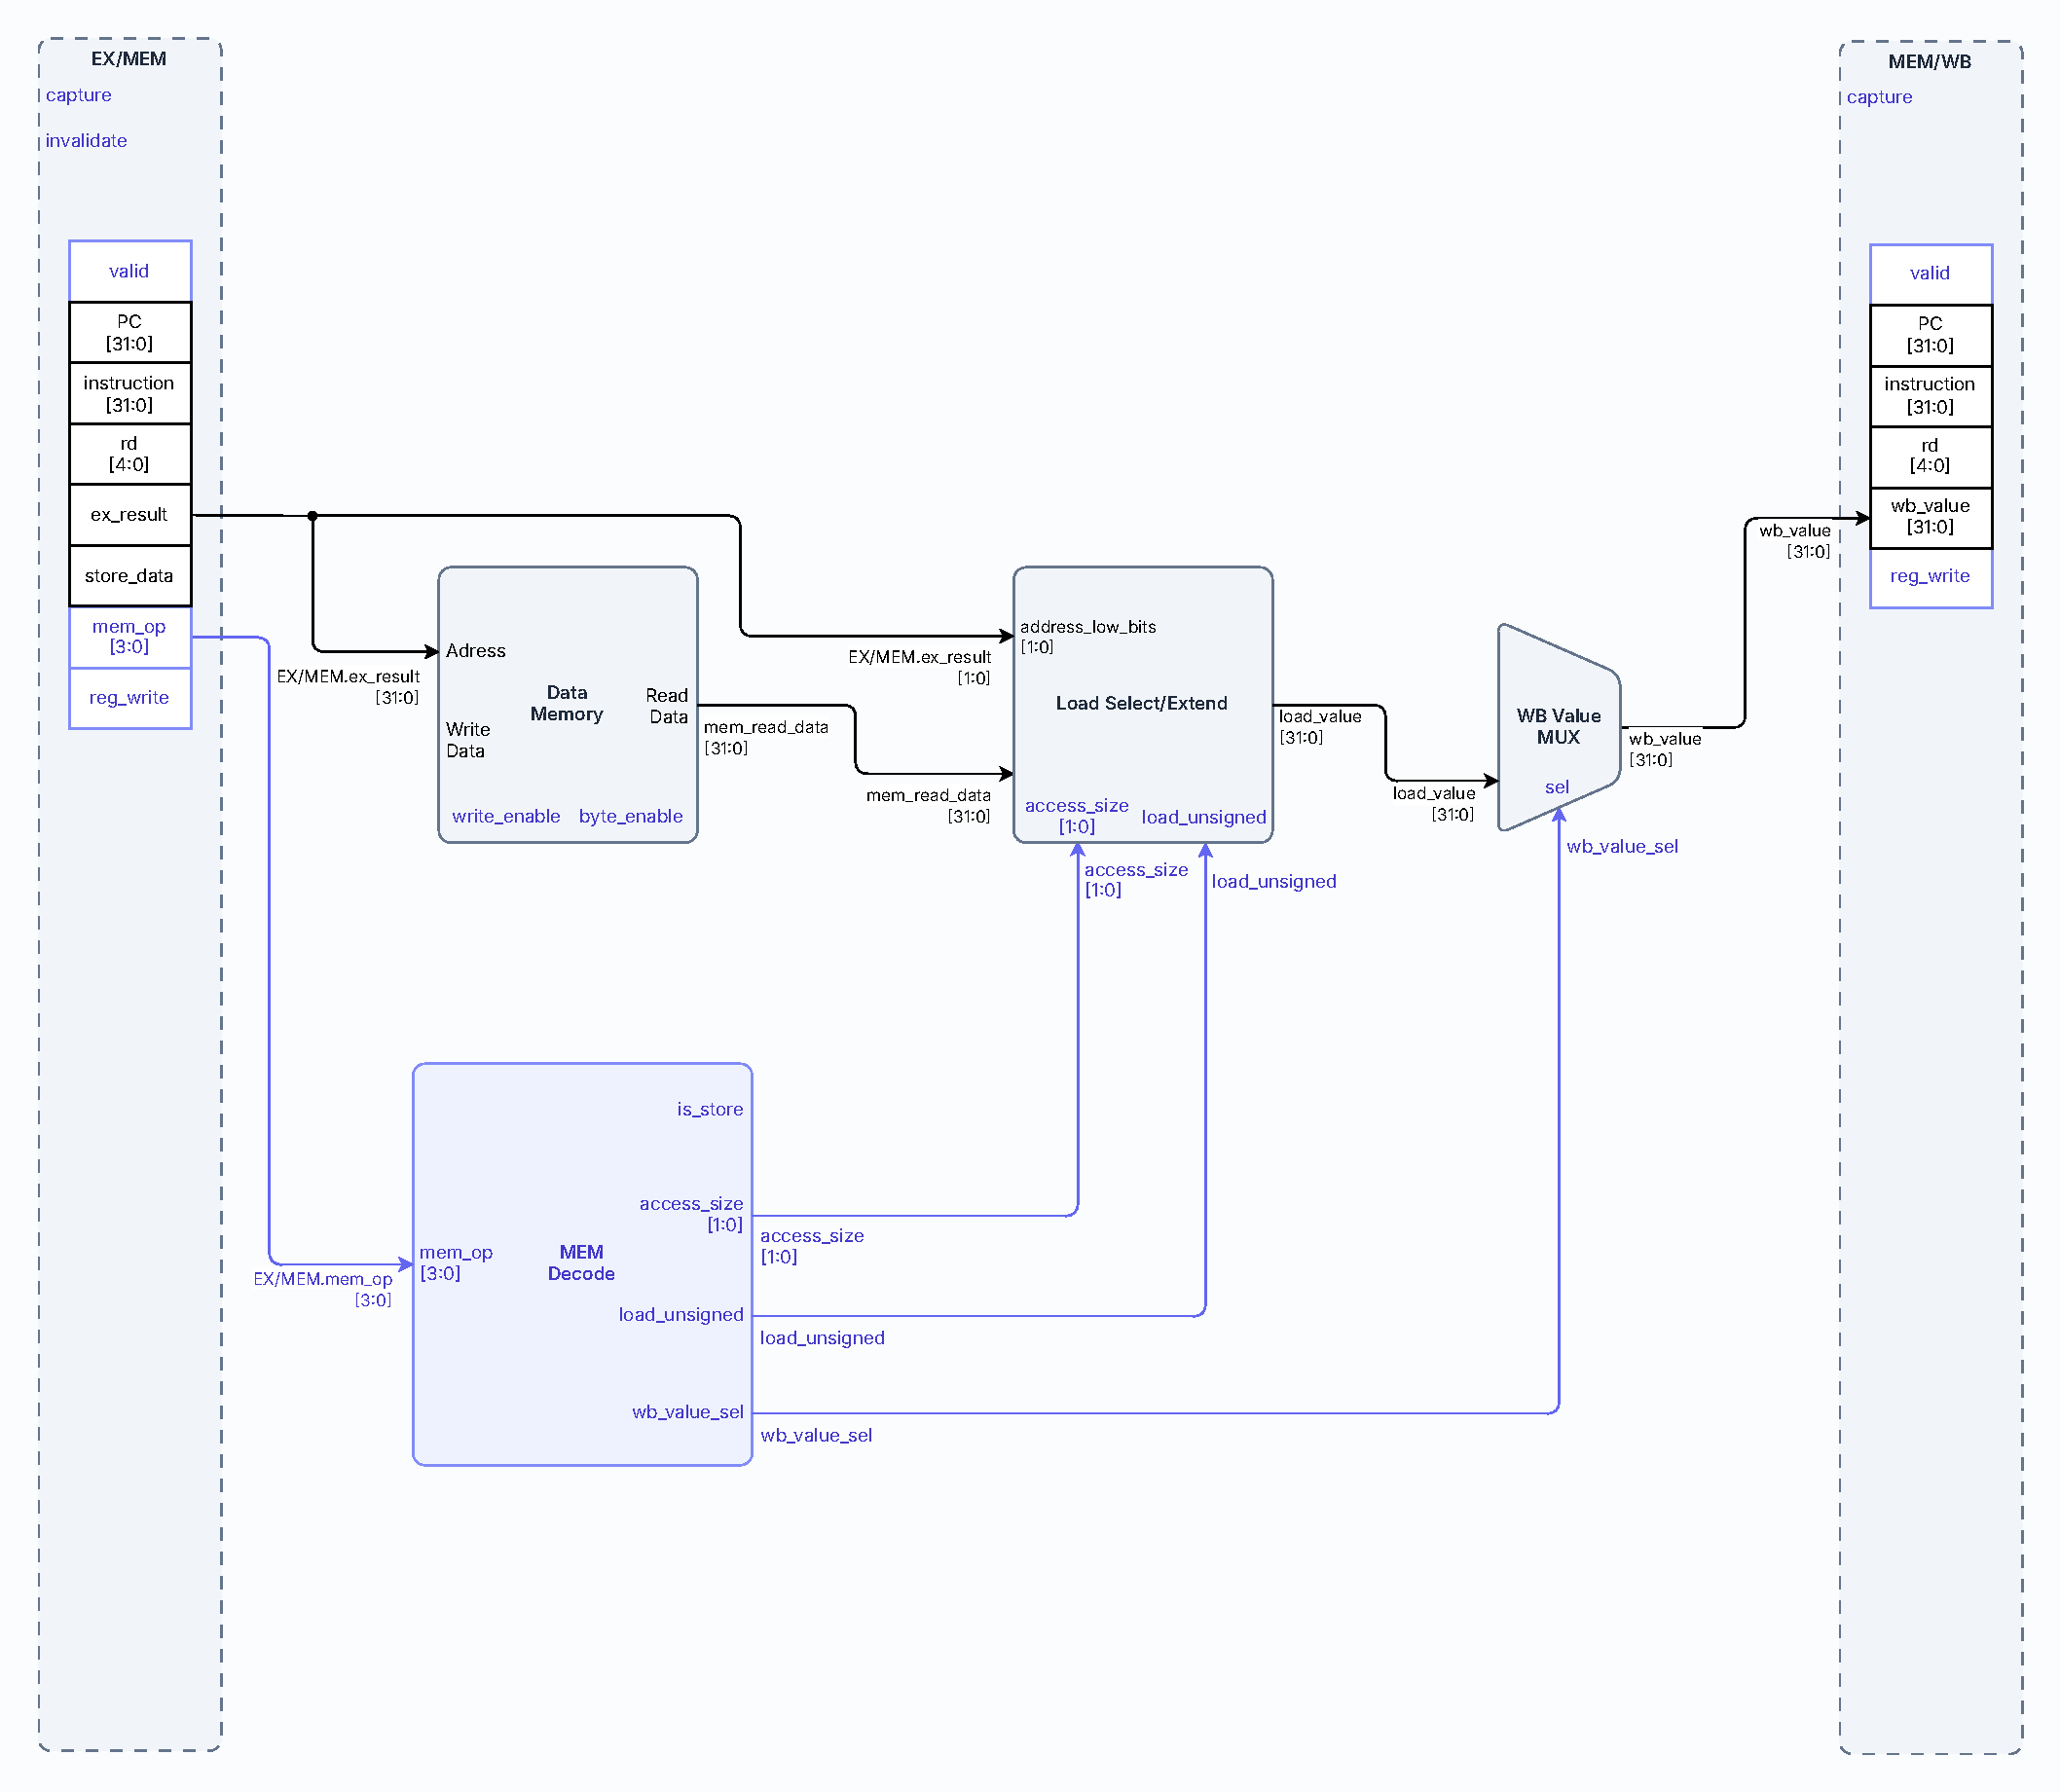
\includegraphics[width=0.72\textwidth]{mem-load.pdf}
  \caption{Recorrido de un load en MEM: lectura de DMEM, selección de bytes y
  extensión del resultado.}
  \label{fig:mem-load}
\end{figure}

\subsubsection{Escritura mediante stores}

Un store llega a MEM con la dirección efectiva y el dato que debe almacenar.
Según la instrucción, el control genera una máscara de cuatro bits que indica
cuántos bytes bajos del dato se escribirán: uno para \code{SB}, dos para
\code{SH} y cuatro para \code{SW}.

DMEM utiliza los dos bits inferiores de la dirección para ubicar esos bytes y
la máscara en los lanes correspondientes. Por ejemplo, un \code{SB} en la
dirección \code{0x05} escribe el byte menos significativo del dato en el
lane 1 de la fila 1. En el flanco autorizado se actualizan juntos los datos y
las marcas de los lanes seleccionados, mientras que los demás conservan su
contenido y validez.

Todos los bytes de un store válido se escriben en el mismo flanco. Además, la
marca se activa incluso cuando el valor escrito es cero, ya que registra si el
byte fue utilizado durante la sesión. La figura~\ref{fig:mem-store} muestra el
recorrido de la dirección, el dato y la máscara hasta su escritura en DMEM.

\begin{figure}[H]
  \centering
  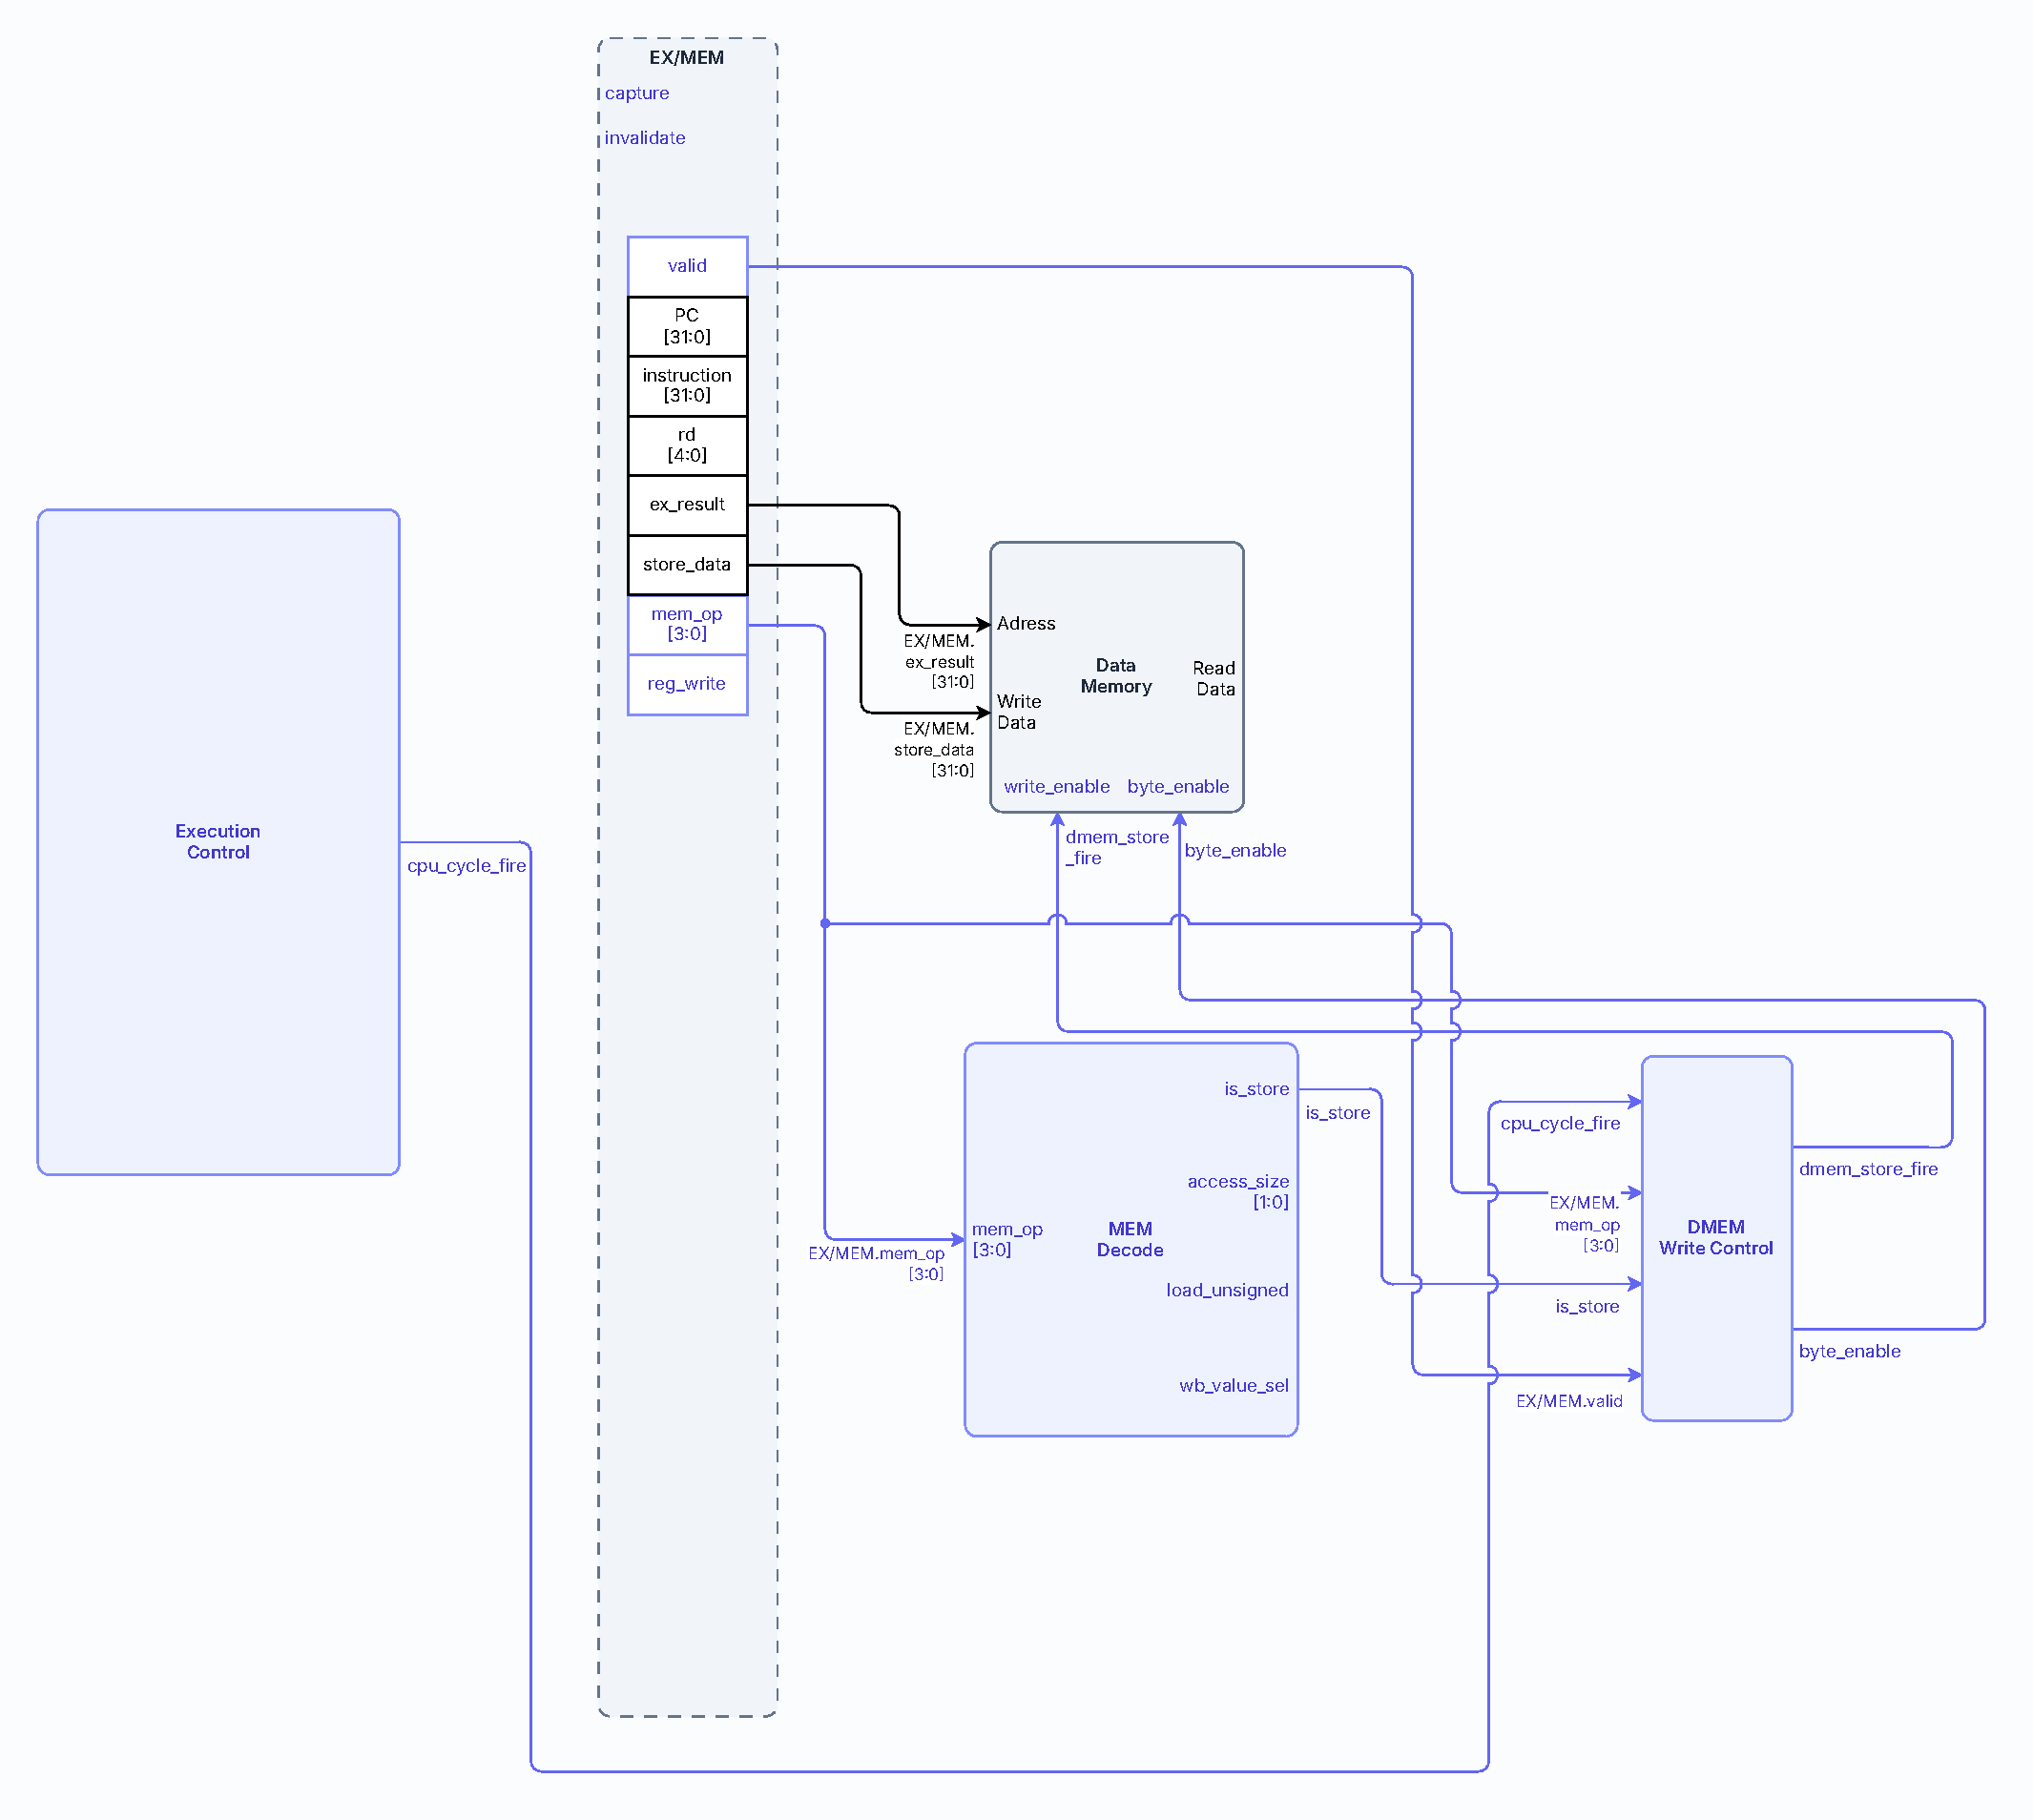
\includegraphics[width=0.72\textwidth]{mem-store.pdf}
  \caption{Recorrido de un store en MEM: dirección, dato, máscara de bytes y
  actualización conjunta de dato y validez.}
  \label{fig:mem-store}
\end{figure}

\section{Direcciones, alineación y rango}

Para que un acceso sea válido, su dirección debe cumplir la alineación exigida
por el tamaño de la operación y todos los bytes solicitados deben pertenecer a
la región permitida. En los loads y stores, estas comprobaciones se realizan
en EX sobre la dirección efectiva. Para el fetch se valida el PC y la región
de la imagen ejecutable, como se explicó en la sección de IMEM.

\subsection{Dirección efectiva}

La dirección efectiva de un load o store se obtiene sumando el valor efectivo
de \code{rs1} y el inmediato de la instrucción. La suma utiliza aritmética de
32 bits, por lo que conserva sus 32 bits inferiores:

\begin{codebox}
effective_address = (rs1_effective + immediate) mod 2^32
\end{codebox}

Por ejemplo, si \code{rs1} vale \code{0xffffffff} y el inmediato es 1, la
dirección resultante es \code{0x00000000}. El acarreo de esta suma no produce
un fault por sí mismo; la dirección resultante se utiliza para comprobar la
alineación y el rango.

\subsection{Alineación}

Los accesos de varios bytes deben comenzar en una dirección múltiplo de su
tamaño. Por eso, un acceso de dos bytes comienza en una dirección par y uno de
cuatro bytes, en una dirección múltiplo de cuatro. El fetch también requiere
un PC alineado a cuatro bytes. La tabla~\ref{tab:alineacion} resume estas
condiciones:

\begin{table}[H]
  \centering
  \small
  \begin{tabular}{ll}
    \toprule
    \textbf{Acceso} & \textbf{Condición} \\
    \midrule
    \code{LB}, \code{LBU}, \code{SB} & sin restricción adicional \\
    \code{LH}, \code{LHU}, \code{SH} & \code{address[0] = 0} \\
    \code{LW}, \code{SW} & \code{address[1:0] = 00} \\
    fetch & \code{PC[1:0] = 00} \\
    \bottomrule
  \end{tabular}
  \caption{Condiciones de alineación.}
  \label{tab:alineacion}
\end{table}

\subsection{Rango del acceso}

Además de estar alineado, un load o store debe tener todos sus bytes dentro de
DMEM. Si la dirección efectiva es el primer byte y \code{N} es el tamaño del
acceso en bytes, se comprueba que el extremo posterior a la región no supere
la capacidad de la memoria:

\begin{codebox}
dmem_range_valid =
    ({1'b0, effective_address} + N) <= DMEM_CAPACITY_BYTES
\end{codebox}

Esta suma y la comparación se realizan con 33 bits para conservar el posible
acarreo al calcular el extremo. Así, una región que supera el límite de las
direcciones de 32 bits no se confunde con una región ubicada al comienzo de la
memoria. Por ejemplo, en una DMEM de 2048 bytes, una palabra que comienza en
la dirección 2044 ocupa los últimos cuatro bytes y está dentro del rango,
mientras que una palabra que comienza en 2048 queda fuera de él.

\subsection{Accesos inválidos}

Una dirección desalineada genera un fault de alineación y una región fuera de
rango genera un fault de acceso. Si una misma operación incumple ambas
condiciones, se informa la desalineación. Cuando hay faults de instrucciones
distintas, prevalece el de la instrucción anterior en el programa. En particular,
un store inválido no modifica datos ni marcas, por lo que no deja una escritura
parcial.

\section{Temporización y acceso a las memorias}

\subsection{Temporización de lectura y escritura}

Las lecturas de IMEM y DMEM son combinacionales: a partir de la dirección
presentada, el dato queda disponible durante el mismo ciclo. Las escrituras,
en cambio, son síncronas y actualizan la memoria en el flanco de reloj cuando
están habilitadas. Como ambas memorias son independientes, IF puede leer una
instrucción mientras MEM accede a datos en ese mismo ciclo.

Este esquema permite que la CPU utilice las memorias sin esperar una respuesta
de latencia variable ni insertar un stall específico por memoria. Cuando el
pipeline está en \code{HOLD}, no se autorizan ciclos de CPU y un store retenido
en MEM no repite su escritura. El reset también inhibe las escrituras.

\subsection{Coordinación de los accesos}

Además de la CPU, otros bloques utilizan las memorias para cargar el programa,
preparar la sesión y observar sus datos. El control del sistema coordina esos
accesos según la actividad en curso, como muestra la
tabla~\ref{tab:ownership}.

\begin{table}[H]
  \centering
  \small
  \begin{tabularx}{\textwidth}{L{1.6cm}L{3.1cm}Y}
    \toprule
    \textbf{Memoria} & \textbf{Bloque} & \textbf{Acceso} \\
    \midrule
    IMEM & Loader & Escribe la imagen durante la carga. \\ \addlinespace
    IMEM & CPU & Lee instrucciones durante la ejecución. \\ \addlinespace
    DMEM & Preparación & Limpia las marcas de validez al iniciar una sesión. \\ \addlinespace
    DMEM & CPU & Lee o escribe datos durante la ejecución. \\ \addlinespace
    DMEM & Debug & Lee datos y marcas cuando la CPU no ejecuta ciclos. \\
    \bottomrule
  \end{tabularx}
  \caption{Bloques que acceden a las memorias y función de cada acceso.}
  \label{tab:ownership}
\end{table}

Estos accesos se coordinan por etapas de funcionamiento. Durante la carga, el
\code{Loader} escribe IMEM y la CPU no ejecuta instrucciones. Luego, la
preparación limpia las marcas de DMEM antes de iniciar la sesión. Durante la
ejecución, la CPU utiliza ambas memorias; cuando Debug necesita observar DMEM,
la CPU queda detenida y un selector presenta la dirección de Debug al camino de
lectura compartido. Así, cada bloque accede a la memoria cuando le corresponde
y se evitan accesos incompatibles sobre una misma memoria.

\section{Perfiles y parametrización}

Las capacidades de IMEM y DMEM se configuran por separado antes de elaborar el
diseño. Cada una se expresa en bytes y determina el rango de direcciones de su
memoria. El dominio arquitectónico admite capacidades entre 4 y $2^{32}$ bytes,
siempre que sean múltiplos de cuatro, ya que las memorias se organizan en
palabras o filas de cuatro bytes.

Los anchos de los índices se calculan a partir de la capacidad configurada y
conservan al menos un bit, incluso para la configuración mínima. La
tabla~\ref{tab:perfiles} presenta los dos perfiles utilizados en el proyecto:

\begin{table}[H]
  \centering
  \small
  \begin{tabular}{lrrl}
    \toprule
    \textbf{Perfil} & \textbf{IMEM} & \textbf{DMEM} & \textbf{Alcance} \\
    \midrule
    \code{REFERENCE} & \SI{1024}{\byte} & \SI{2048}{\byte} &
    Simulación, síntesis, implementación y placa. \\
    \code{ALT_1000} & \SI{1000}{\byte} & \SI{1000}{\byte} &
    Elaboración y simulaciones de parametrización. \\
    \bottomrule
  \end{tabular}
  \caption{Perfiles de memoria.}
  \label{tab:perfiles}
\end{table}

\code{REFERENCE} es el perfil utilizado para la implementación en FPGA, mientras
que \code{ALT_1000} se usa en simulación para comprobar la parametrización con
capacidades que no son potencias de dos. La PC y la FPGA deben utilizar el
mismo perfil para interpretar los límites de las memorias de forma coherente.

Una configuración fuera del dominio arquitectónico se rechaza antes de
elaborar los arrays. Si una capacidad es válida para la arquitectura, pero una
realización concreta no puede admitirla, se informa como error de
configuración y no como un fault del programa.

\section{Reprogramación y estado inicial}

Una vez configurada la FPGA, el sistema puede ejecutar distintos programas sin
modificar el diseño del procesador. Para cambiar de programa, la PC envía una
nueva imagen de instrucciones mediante el comando \code{LOAD} y el sistema la
almacena en IMEM. Así, la reprogramación cambia el contenido que ejecuta la
CPU sin resintetizar el diseño ni volver a cargar el bitstream.

La imagen y la sesión representan dos aspectos distintos de la ejecución: la
imagen contiene las instrucciones cargadas, mientras que la sesión comprende
una ejecución de esas instrucciones y el estado que se va generando en el
procesador y en DMEM. Una misma imagen puede ejecutarse en más de una sesión,
siempre que se prepare nuevamente el estado inicial antes de comenzar.

Cuando se acepta una nueva carga, el sistema abandona la sesión vigente e
invalida la imagen anterior. El \code{Loader} escribe entonces la nueva imagen
en IMEM y, una vez recibida, comienza la preparación de la sesión. Esta etapa
establece el estado inicial desde el que se ejecutará el programa:

\begin{itemize}
  \item \code{PC = 0};
  \item banco de registros en cero lógico;
  \item registros interetapa inválidos;
  \item DMEM con todas sus marcas de validez en cero;
  \item \code{cycle_count = 0};
  \item metadatos de fault sin vigencia.
\end{itemize}

Al limpiar las marcas de DMEM, la preparación garantiza que la nueva sesión
observe cero en las posiciones que todavía no escribió, aunque el almacenamiento
conserve datos de la sesión anterior. Del mismo modo, solo los bytes confirmados
de la nueva imagen se consideran instrucciones ejecutables.

Una vez completadas la carga y la preparación, la imagen se publica y queda
disponible para ejecutar. La secuencia completa se describe en
\doc{architecture/session/execution_control.md}{Control de ejecución y sesión}.
